% ============================================================================
% CHAPTER 1I: INDUSTRIAL AND COMPUTER SYSTEMS
% ============================================================================

\section{Industrial and Computer Systems}
\label{sec:industrial_computer}

This section covers systems from manufacturing, process control, and computer science---domains where control theory meets discrete events, queueing, and information flow.

% ============================================================================
\subsection{Industrial Process Control}
\label{subsec:industrial_process}
% ============================================================================

\subsubsection{Conveyor Belt System}

\begin{figure}[htbp]
\centering
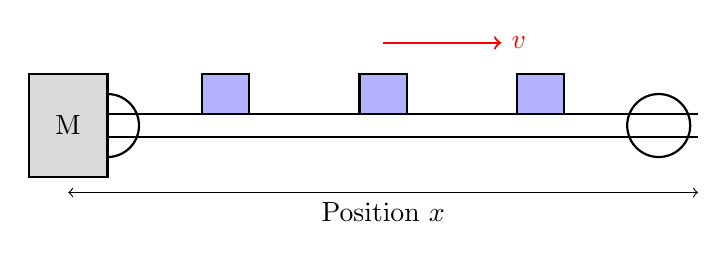
\begin{tikzpicture}
    % Belt
    \draw[thick] (0,0) -- (8,0);
    \draw[thick] (0,0.3) -- (8,0.3);

    % Rollers
    \draw[thick] (0.5,0.15) circle (0.4);
    \draw[thick] (7.5,0.15) circle (0.4);

    % Motor
    \draw[thick, fill=gray!30] (-0.5,-0.5) rectangle (0.5,0.8);
    \node at (0,0.15) {M};

    % Items on belt
    \foreach \x in {2,4,6} {
        \draw[thick, fill=blue!30] (\x-0.3,0.3) rectangle (\x+0.3,0.8);
    }

    % Speed
    \draw[->, thick, red] (4,1.2) -- (5.5,1.2) node[right] {$v$};

    % Position
    \draw[<->] (0,-0.7) -- (8,-0.7) node[midway, below] {Position $x$};
\end{tikzpicture}
\caption{Conveyor belt system with motor drive.}
\label{fig:conveyor}
\end{figure}

Motor-driven conveyor dynamics:
\begin{equation}
J_{\text{eq}}\dot{\omega} + B\omega = K_t i - \tau_L
\end{equation}

where $J_{\text{eq}}$ includes reflected inertia of belt and load.

Belt velocity: $v = r\omega$ where $r$ is the drive roller radius.

Transfer function (speed control):
\begin{equation}
\frac{V(s)}{I(s)} = \frac{rK_t}{J_{\text{eq}}s + B}
\end{equation}

\subsubsection{Temperature Control Zone}

Industrial ovens often have multiple zones:

\begin{figure}[htbp]
\centering
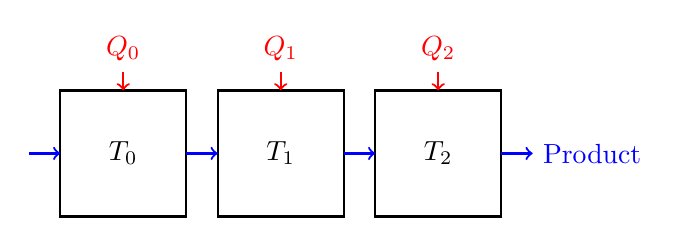
\begin{tikzpicture}[scale=0.8]
    % Zones
    \foreach \i in {0,1,2} {
        \draw[thick] (\i*2.5,0) rectangle (\i*2.5+2,2);
        \node at (\i*2.5+1,1) {$T_\i$};
        \draw[->, thick, red] (\i*2.5+1,2.3) -- (\i*2.5+1,2) node[above, pos=0] {$Q_\i$};
    }

    % Product flow
    \draw[->, thick, blue] (-0.5,1) -- (0,1);
    \draw[->, thick, blue] (2,1) -- (2.5,1);
    \draw[->, thick, blue] (4.5,1) -- (5,1);
    \draw[->, thick, blue] (7,1) -- (7.5,1) node[right] {Product};
\end{tikzpicture}
\caption{Multi-zone temperature control.}
\label{fig:temp_zones}
\end{figure}

Each zone:
\begin{equation}
C_i\frac{\dd T_i}{\dd t} = Q_i - \frac{T_i - T_{i-1}}{R_{i-1,i}} - \frac{T_i - T_{i+1}}{R_{i,i+1}} - \frac{T_i - T_{\infty}}{R_{i,\infty}}
\end{equation}

% ============================================================================
\subsection{Robotic Manipulators}
\label{subsec:robotics}
% ============================================================================

\subsubsection{Single-Link Robot Arm}

\begin{figure}[htbp]
\centering
\begin{tikzpicture}
    % Base
    \fill[pattern=north east lines] (-0.5,-0.3) rectangle (0.5,0);
    \draw[thick] (-0.5,0) -- (0.5,0);

    % Joint
    \draw[thick, fill=gray!30] (0,0) circle (0.3);

    % Link
    \draw[thick, fill=blue!20] (0.2,0.2) -- (3,1.5) -- (3.2,1.3) -- (0.4,0) -- cycle;

    % End effector
    \fill[red] (3.1,1.4) circle (0.15);

    % Angle
    \draw[->] (1,0) arc (0:25:1) node[midway, right] {$\theta$};

    % Length
    \node at (1.8,0.5) {$\ell$};

    % Torque
    \draw[->, thick, green!60!black] (0.5,0.5) arc (45:90:0.5) node[above] {$\tau$};

    % Gravity
    \draw[->, thick] (3.1,1.2) -- (3.1,0.4) node[below] {$mg$};
\end{tikzpicture}
\caption{Single-link robot arm.}
\label{fig:single_link}
\end{figure}

Equation of motion:
\begin{equation}
J\ddot{\theta} + B\dot{\theta} + mg\ell\cos\theta = \tau
\end{equation}

Linearized about horizontal ($\theta_0 = 0$):
\begin{equation}
J\ddot{\theta} + B\dot{\theta} + mg\ell = \tau
\end{equation}

Note: Gravity creates a constant disturbance torque.

\subsubsection{Two-Link Planar Arm}

The dynamics become coupled and nonlinear:
\begin{equation}
\mM(\vecq)\ddot{\vecq} + \mC(\vecq, \dot{\vecq})\dot{\vecq} + \vecg(\vecq) = \boldsymbol{\tau}
\end{equation}

where:
\begin{itemize}
    \item $\mM(\vecq)$ = mass matrix (configuration-dependent)
    \item $\mC(\vecq, \dot{\vecq})$ = Coriolis and centrifugal terms
    \item $\vecg(\vecq)$ = gravity vector
    \item $\boldsymbol{\tau}$ = joint torques
\end{itemize}

For a two-link arm:
\begin{align}
M_{11} &= m_1 \ell_{c1}^2 + m_2(\ell_1^2 + \ell_{c2}^2 + 2\ell_1\ell_{c2}\cos\theta_2) + I_1 + I_2 \\
M_{12} &= m_2(\ell_{c2}^2 + \ell_1\ell_{c2}\cos\theta_2) + I_2 \\
M_{22} &= m_2\ell_{c2}^2 + I_2
\end{align}

% ============================================================================
\subsection{CNC Machine Tools}
\label{subsec:cnc}
% ============================================================================

\subsubsection{Axis Drive Model}

Each axis of a CNC machine:
\begin{equation}
J_{\text{axis}}\ddot{x} + B\dot{x} + F_c\sgn(\dot{x}) = F_{\text{motor}} - F_{\text{cut}}
\end{equation}

where $F_c$ is Coulomb friction and $F_{\text{cut}}$ is cutting force disturbance.

\subsubsection{Servo System}

Position loop transfer function:
\begin{equation}
\frac{X(s)}{X_{\text{cmd}}(s)} = \frac{K_p K_v/s}{1 + K_p K_v/s + s^2/\omega_n^2} \approx \frac{K_p}{\tau_p s + 1}
\end{equation}

for well-tuned systems where $K_v = K_p/\tau_p$.

% ============================================================================
\subsection{Power Systems}
\label{subsec:power_systems}
% ============================================================================

\subsubsection{Synchronous Generator}

Swing equation:
\begin{equation}
\frac{2H}{\omega_s}\frac{\dd^2\delta}{\dd t^2} + D\frac{\dd\delta}{\dd t} = P_m - P_e
\end{equation}

where:
\begin{itemize}
    \item $H$ = inertia constant (seconds)
    \item $\delta$ = rotor angle (electrical radians)
    \item $\omega_s$ = synchronous speed
    \item $P_m$ = mechanical power
    \item $P_e$ = electrical power
\end{itemize}

Linearized about operating point:
\begin{equation}
\frac{\Delta\delta(s)}{\Delta P_m(s)} = \frac{\omega_s/2H}{s^2 + (D\omega_s/2H)s + K_s\omega_s/2H}
\end{equation}

where $K_s = \partial P_e/\partial\delta$ is the synchronizing coefficient.

\subsubsection{Automatic Generation Control (AGC)}

Area control error:
\begin{equation}
\text{ACE} = \Delta P_{\text{tie}} + B\Delta f
\end{equation}

where $B$ is the frequency bias setting.

% ============================================================================
\subsection{Queueing Systems}
\label{subsec:queueing}
% ============================================================================

\subsubsection{M/M/1 Queue}

\begin{figure}[htbp]
\centering
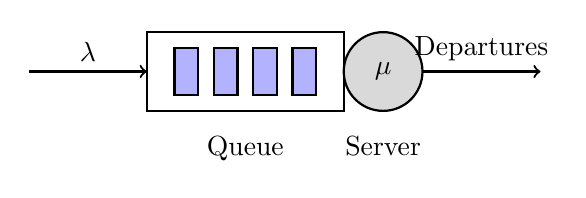
\begin{tikzpicture}
    % Arrivals
    \draw[->, thick] (0,0) -- (1.5,0) node[above, midway] {$\lambda$};

    % Queue
    \draw[thick] (1.5,-0.5) rectangle (4,0.5);
    \foreach \x in {2,2.5,3,3.5} {
        \draw[thick, fill=blue!30] (\x-0.15,-0.3) rectangle (\x+0.15,0.3);
    }
    \node[below] at (2.75,-0.7) {Queue};

    % Server
    \draw[thick, fill=gray!30] (4.5,0) circle (0.5);
    \node at (4.5,0) {$\mu$};
    \node[below] at (4.5,-0.7) {Server};

    % Departures
    \draw[->, thick] (5,0) -- (6.5,0) node[above, midway] {Departures};
\end{tikzpicture}
\caption{M/M/1 queue model.}
\label{fig:mm1_queue}
\end{figure}

Steady-state:
\begin{align}
\text{Utilization:} \quad \rho &= \lambda/\mu \\
\text{Mean queue length:} \quad L &= \frac{\rho}{1-\rho} \\
\text{Mean waiting time:} \quad W &= \frac{1}{\mu - \lambda}
\end{align}

\subsubsection{Fluid Flow Model}

For control design, queues can be approximated as fluid:
\begin{equation}
\frac{\dd q}{\dd t} = \lambda(t) - \mu(t)
\end{equation}

where $q$ is queue length, $\lambda$ is arrival rate, and $\mu$ is service rate.

Transfer function:
\begin{equation}
\frac{Q(s)}{\Lambda(s) - M(s)} = \frac{1}{s}
\end{equation}

% ============================================================================
\subsection{Computer Systems}
\label{subsec:computer_systems}
% ============================================================================

\subsubsection{CPU Load Control}

CPU utilization dynamics:
\begin{equation}
\tau\frac{\dd U}{\dd t} + U = K_u \cdot R
\end{equation}

where $U$ is utilization, $R$ is admission rate, and $\tau$ depends on job service time.

\subsubsection{Network Congestion Control}

TCP congestion window dynamics (simplified):
\begin{equation}
\frac{\dd W}{\dd t} = \frac{1}{RTT} - \frac{W}{2} \cdot p
\end{equation}

where $W$ is congestion window, $RTT$ is round-trip time, and $p$ is packet loss probability.

\subsubsection{Memory Management}

Page fault rate model:
\begin{equation}
f = f_0 \left(\frac{W_s}{M}\right)^\alpha
\end{equation}

where $M$ is allocated memory, $W_s$ is working set size, and $\alpha$ is a workload parameter.

% ============================================================================
\subsection{Data Center Thermal Management}
\label{subsec:datacenter}
% ============================================================================

\begin{figure}[htbp]
\centering
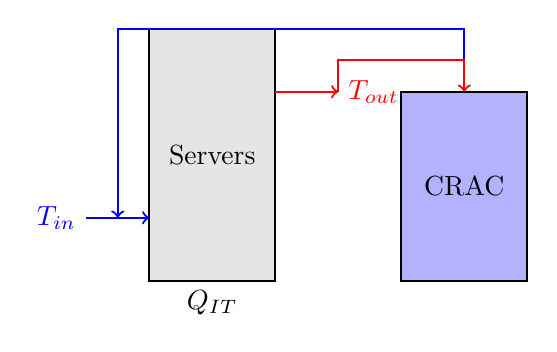
\begin{tikzpicture}[scale=0.8]
    % Server rack
    \draw[thick, fill=gray!20] (0,0) rectangle (2,4);
    \node at (1,2) {Servers};
    \node[below] at (1,0) {$Q_{\text{IT}}$};

    % Air flow
    \draw[->, thick, blue] (-1,1) -- (0,1) node[left, pos=0] {$T_{\text{in}}$};
    \draw[->, thick, red] (2,3) -- (3,3) node[right] {$T_{\text{out}}$};

    % CRAC unit
    \draw[thick, fill=blue!30] (4,0) rectangle (6,3);
    \node at (5,1.5) {CRAC};

    % Cooling
    \draw[->, thick, blue] (5,3) -- (5,4) -- (-0.5,4) -- (-0.5,1);
    \draw[->, thick, red] (3,3) -- (3,3.5) -- (5,3.5) -- (5,3);
\end{tikzpicture}
\caption{Data center thermal model.}
\label{fig:datacenter_thermal}
\end{figure}

Thermal dynamics:
\begin{equation}
C_{\text{room}}\frac{\dd T}{\dd t} = Q_{\text{IT}} - \dot{m}c_p(T - T_{\text{supply}})
\end{equation}

where $\dot{m}$ is air mass flow rate (controlled by CRAC fans).

% ============================================================================
\subsection{Building Automation}
\label{subsec:building}
% ============================================================================

\subsubsection{HVAC Zone Model}

\begin{equation}
C_z\frac{\dd T_z}{\dd t} = Q_{\text{HVAC}} + Q_{\text{internal}} + Q_{\text{solar}} - UA(T_z - T_{\text{out}})
\end{equation}

Transfer function from HVAC power to zone temperature:
\begin{equation}
\frac{T_z(s)}{Q_{\text{HVAC}}(s)} = \frac{1/UA}{\tau s + 1}
\end{equation}

where $\tau = C_z/UA$.

\subsubsection{Lighting Control}

Dimming dynamics:
\begin{equation}
\tau_L\frac{\dd L}{\dd t} + L = K_L \cdot d
\end{equation}

where $L$ is light level, $d$ is dimmer setting, and $\tau_L$ is lamp response time.

% ============================================================================
\subsection{Traffic Flow}
\label{subsec:traffic}
% ============================================================================

\subsubsection{Cell Transmission Model}

For a road segment:
\begin{equation}
\frac{\dd n_i}{\dd t} = q_{i-1} - q_i
\end{equation}

where $n_i$ is vehicle count in cell $i$ and $q_i$ is flow rate.

Flow-density relationship:
\begin{equation}
q = v_f n \left(1 - \frac{n}{n_{\max}}\right)
\end{equation}

\subsubsection{Traffic Signal Timing}

Green time allocation affects queue discharge:
\begin{equation}
\frac{\dd q}{\dd t} = \lambda - s \cdot g(t)
\end{equation}

where $s$ is saturation flow rate and $g(t) \in \{0, 1\}$ indicates green signal.

% ============================================================================
\subsection{Exercises: Industrial and Computer Systems}
% ============================================================================

\begin{exercise}
A conveyor belt has equivalent inertia $J = 2$ kg$\cdot$m$^2$, friction $B = 0.5$ N$\cdot$m$\cdot$s/rad, drive roller radius $r = 0.1$ m, and motor constant $K_t = 0.5$ N$\cdot$m/A.
\begin{enumerate}[label=(\alph*)]
    \item Find the transfer function from motor current to belt velocity
    \item Calculate the current needed for 0.5 m/s belt speed
    \item Find the time constant
\end{enumerate}
\end{exercise}

\begin{exercise}
A single-link robot arm has $J = 0.5$ kg$\cdot$m$^2$, $B = 0.1$ N$\cdot$m$\cdot$s/rad, $m = 2$ kg, and $\ell = 0.5$ m.
\begin{enumerate}[label=(\alph*)]
    \item Write the nonlinear equation of motion
    \item Linearize about $\theta_0 = 0$ (horizontal)
    \item Find the gravity compensation torque
    \item Derive the transfer function from torque to angle (with gravity compensated)
\end{enumerate}
\end{exercise}

\begin{exercise}
An M/M/1 queue has arrival rate $\lambda = 80$ jobs/s and service rate $\mu = 100$ jobs/s.
\begin{enumerate}[label=(\alph*)]
    \item Calculate the utilization
    \item Find the mean queue length
    \item Find the mean response time (waiting + service)
    \item If the arrival rate increases to 90 jobs/s, how do the metrics change?
\end{enumerate}
\end{exercise}

\begin{exercise}
A data center has thermal capacitance $C = 10^6$ J/K, heat load $Q_{\text{IT}} = 100$ kW, and air flow rate that removes heat according to $\dot{Q}_{\text{cool}} = 5000(T - 18)$ W where $T$ is in °C.
\begin{enumerate}[label=(\alph*)]
    \item Find the steady-state temperature
    \item Calculate the thermal time constant
    \item If IT load suddenly increases to 120 kW, find the new steady-state and time to reach it
\end{enumerate}
\end{exercise}

\begin{exercise}
A traffic intersection has arrival rate 600 vehicles/hour and saturation flow 1800 vehicles/hour. The cycle length is 90 seconds.
\begin{enumerate}[label=(\alph*)]
    \item Find the minimum green time to prevent queue buildup
    \item If green time is 40 seconds, calculate the average queue at the start of green
    \item Model the queue dynamics as a hybrid system
\end{enumerate}
\end{exercise}
